\documentclass[11pt,a4paper]{article}
\usepackage[margin=2cm]{geometry}
\usepackage{graphicx,booktabs,amsmath,amssymb,xcolor,hyperref,float,enumitem,longtable}
\hypersetup{colorlinks=true,linkcolor=blue!50!black,urlcolor=blue!50!black}
\newcommand{\plain}[1]{\par\noindent\colorbox{blue!6}{\parbox{\dimexpr\linewidth-2\fboxsep}{\textbf{In plain words.} #1}}\par\medskip}
\newcommand{\ok}{\textcolor{green!50!black}{\textbf{Succeeded}}}
\newcommand{\no}{\textcolor{red!70!black}{\textbf{Failed}}}
\newcommand{\mixed}{\textcolor{orange!80!black}{\textbf{Mixed}}}
\title{Where the Shortcut Sits --- Full Project Report\\\large Location-dependent failure of ROI masking for in-ROI artifacts, and what to do instead}
\author{Project repository: \url{https://github.com/hossam1999/Where_shortcut_sits}}
\date{27 September 2026}
\begin{document}
\sloppy
\maketitle
\tableofcontents
\newpage

\section{Executive summary}
\plain{Medical AI models often ``cheat'' by looking at things that are not the disease---hair on the skin, measurement
marks drawn by the sonographer, food debris in the gut. The usual fix is to show the model only the lesion (``masking'').
We proved, in four diseases, that this fix fails when the cheating cue sits \emph{on the lesion itself}: masking removes
everything except the cue. We explained why with a simple formula, and we built and tested remedies. The strongest
practical remedy combines masking, a new ``erase'' step that needs no annotation of the artifact, and re-balancing of the
training data; which remedy works best depends on what actually carries the cheating cue.}
\begin{enumerate}[leftmargin=*]
\item \ok\ \textbf{The location effect.} Masking helps far more for artifacts outside the region of interest (ROI)
than inside, in dermoscopy (hair), thyroid and ovarian ultrasound (calipers) and capsule endoscopy (debris): crossover
+0.15 to +0.37 reversed-test AUROC, all significant after Holm correction; replicated on four frozen backbones,
with fine-tuned ResNet-50 and ViT, and robust to the artifact-label definition.
\item \ok\ \textbf{Masking can harm.} When masking also removes disease context it hurts: real dermoscopy hair,
controlled sweeps (ovary $-0.20$, capsule $-0.10$, dermoscopy rulers), capsule fine-tuning ($-0.28$), and on the
\emph{unaltered} thyroid test set ($-0.10$ on shortcut-conflicting cases).
\item \ok\ \textbf{Theory.} One closed-form expression explains all these signs (agreement with simulation 0.009 AUROC).
Fitted only to each model's clean and correlated results, it matches the held-out hard-test results of real models
(average error 0.039 AUROC) and the location gap in 14 dataset/model pairs (correlation 0.997; 13 of 14 signs).
\item \mixed\ \textbf{The remedy (U-MtE).} Works where the artifact is a distinct overlay (thyroid +0.13 to +0.22
over masking on three backbones; +0.14 end-to-end with ResNet-50); erasure beats augmentation (3/4 cohorts); fails when
the artifact resembles the disease (capsule) unless disease-protected, and cannot help when the shortcut lives in
correlates of the artifact (hair, chest drains) --- there label-based reweighting wins.
\item \ok\ \textbf{Foundation models.} The location effect is present in zero-shot vision--language models before any
training; describing the artifact in text and erasing it does not work, our image-side method does.
\item \mixed\ \textbf{One procedure for all cases.} A validation-driven selector beats masking everywhere and matches
the best candidate in each cohort, but is not uniformly better than DFR.
\item \ok\ \textbf{Reproducibility.} Pre-registration before every experiment; the original pilot replicated (73/88
numbers exactly); every table and figure generated by scripts; a two-command public tool.
\end{enumerate}

\section{The question}
\plain{If an AI model learns to recognise a disease from a mark that happens to accompany it, removing everything
except the lesion should stop the cheating---unless the mark is on the lesion. We measure exactly when and how much.}
A \emph{trap} trains a classifier where the artifact accompanies one class 90\% of the time and tests on a reversed
environment where it accompanies the other class 90\% of the time. A model that relies on the artifact collapses on the
reversed test. We compare mitigations by reversed-test AUROC, and always also report correlated and clean AUROC to
detect ``gaming'' (a method that merely flips the shortcut). The overlap $r=|\text{artifact}\cap\text{ROI}|/|\text{artifact}|$
defines in-ROI (Trap A, $r\ge0.5$) and out-of-ROI (Trap B, $r<0.1$) artifacts.

\section{Data and artifacts}
\plain{We used five public medical imaging collections. Below are real examples: the green outline is the region of
interest (lesion, nodule, tumour, lungs) and red marks the artifact the model could cheat with.}
\begin{figure}[H]\centering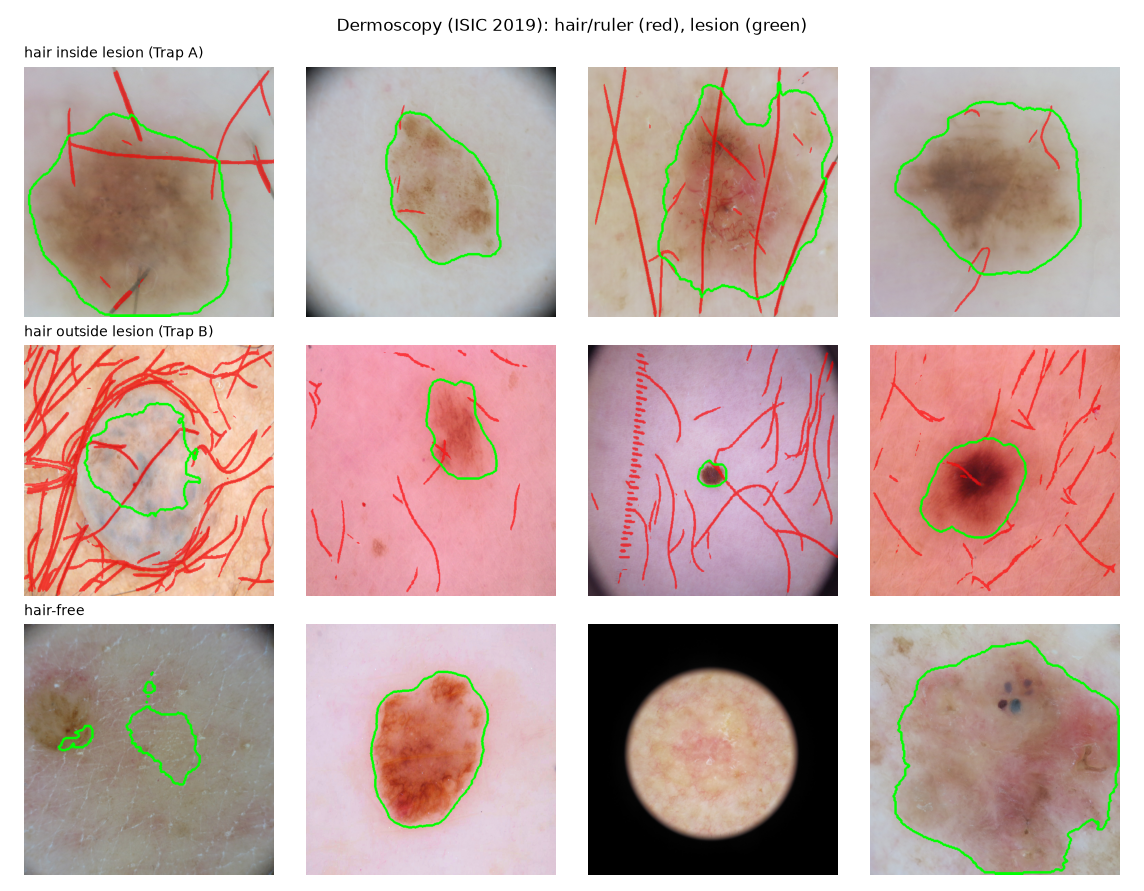
\includegraphics[width=.92\linewidth]{figures/data_isic.png}
\caption{Dermoscopy, ISIC 2019 (25,331 images). Hair and ruler masks from Wegley et al.\ (2026). Note that Trap~B
images can still carry some hair on the lesion: the rule is that less than 10\% of the hair lies inside.}\end{figure}
\begin{figure}[H]\centering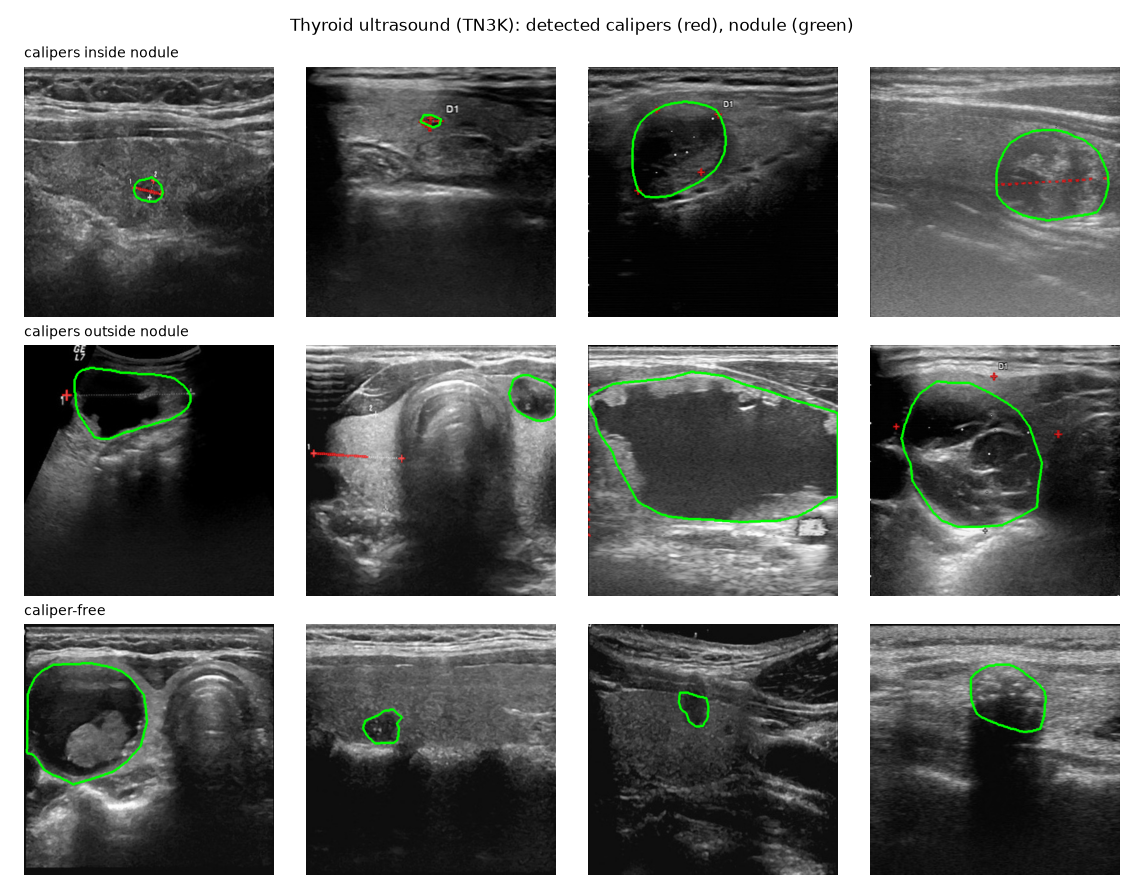
\includegraphics[width=.92\linewidth]{figures/data_thyroid.png}
\caption{Thyroid ultrasound, TN3K with TNCD pathology labels (3,493 images). Calipers found by a frozen rule-based
detector (95\% of detections are real calipers in a 40-image audit).}\end{figure}
\begin{figure}[H]\centering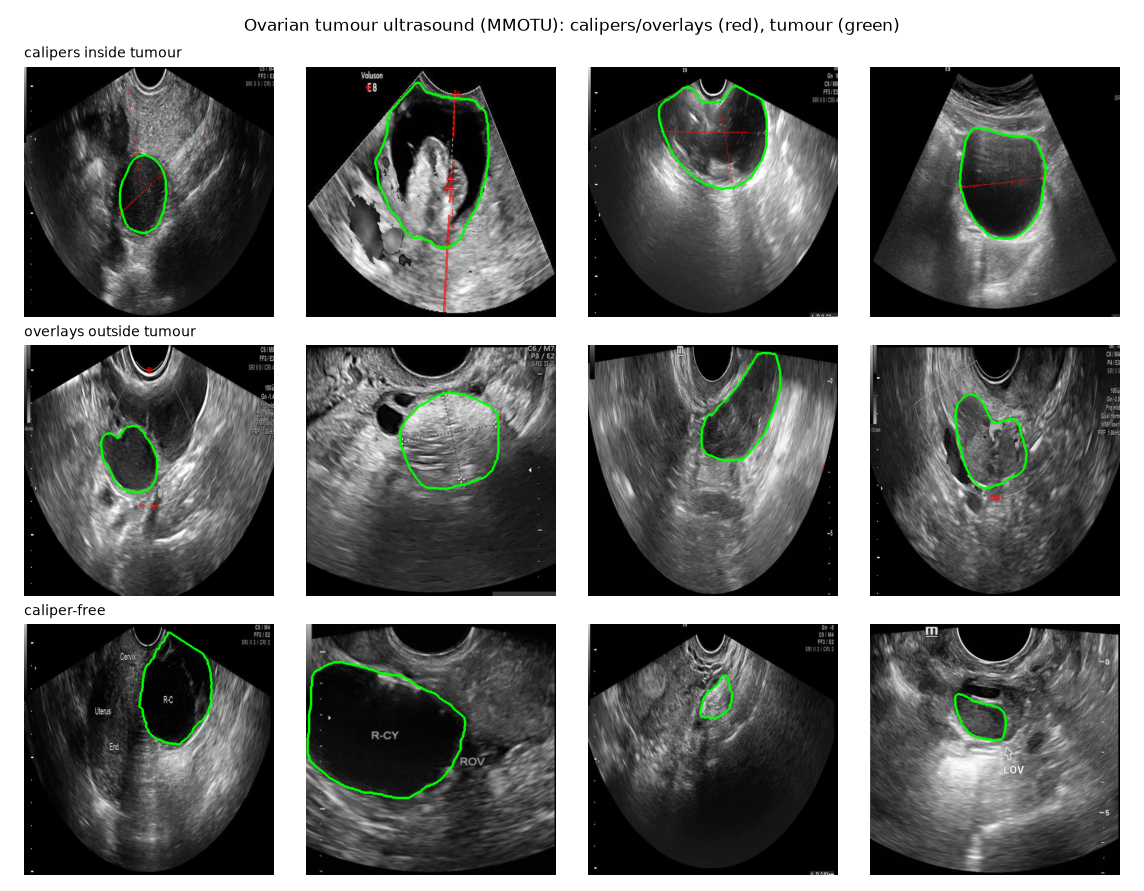
\includegraphics[width=.92\linewidth]{figures/data_ovary.png}
\caption{Ovarian tumour ultrasound, MMOTU (1,202 images; CC BY 4.0). The same detector; ``outside'' detections are
often other on-screen overlays (zoom boxes, focus markers).}\end{figure}
\begin{figure}[H]\centering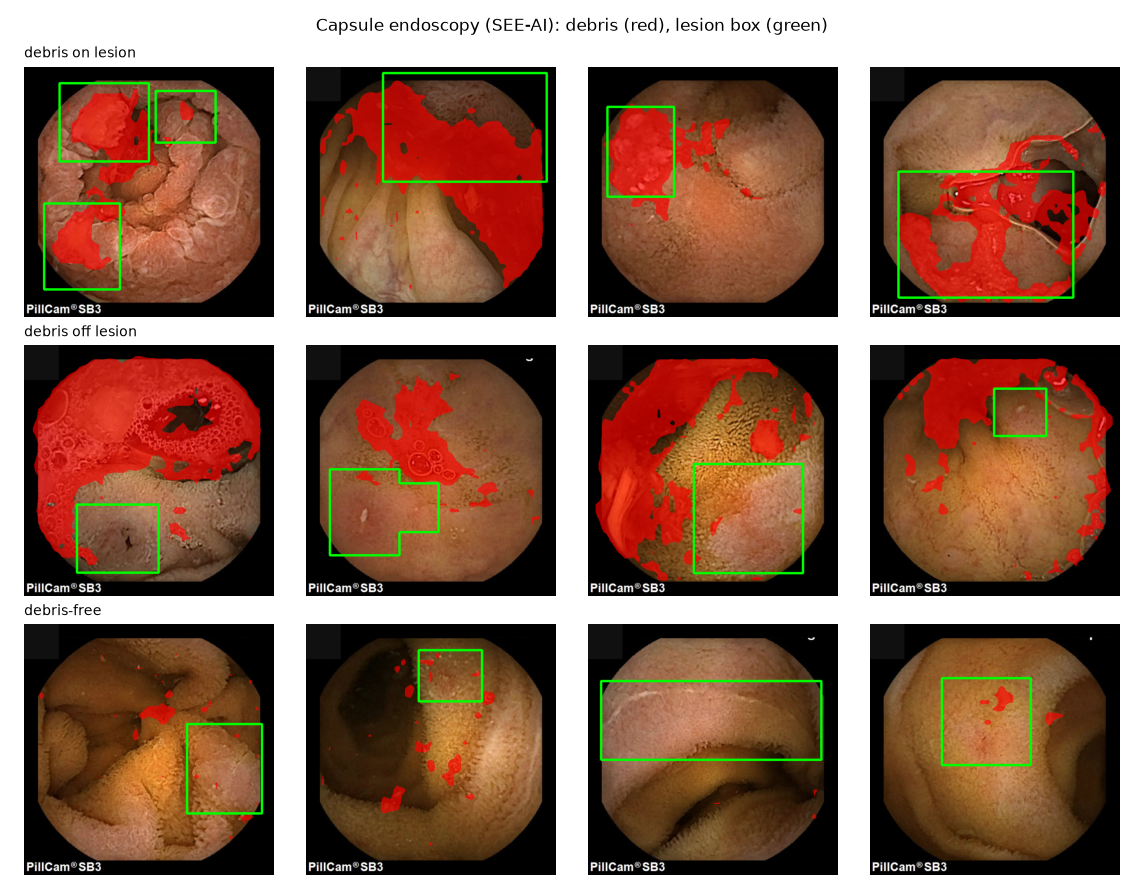
\includegraphics[width=.92\linewidth]{figures/data_capsule.png}
\caption{Capsule endoscopy, SEE-AI (5,481 frames; CC BY 4.0). Debris segmented by a patch-token probe trained on expert
masks (pixel accuracy 0.92, IoU 0.62). Debris can resemble the yellow-white fibrin of erosions.}\end{figure}
\begin{figure}[H]\centering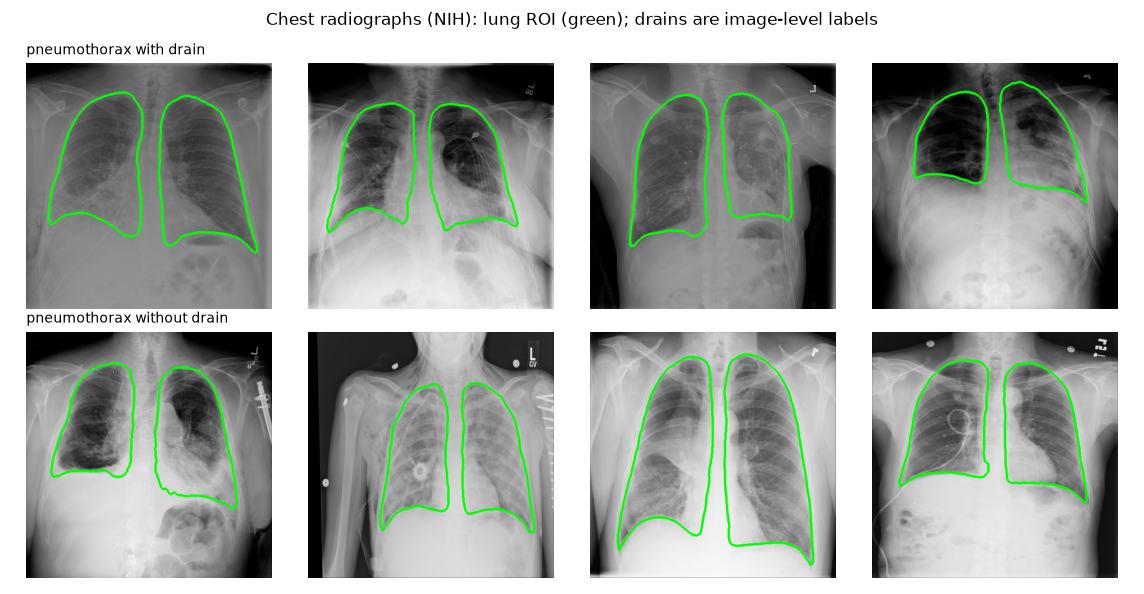
\includegraphics[width=.75\linewidth]{figures/data_cxr.png}
\caption{Chest radiographs, NIH ChestX-ray14. Drains are labelled per image (no pixel masks); they lie inside the
lungs, so only the in-ROI case exists.}\end{figure}
\paragraph{Controlled (synthetic) artifacts --- described, not shown.} To isolate location, the controlled experiments
paste a drawn artifact (ruler for dermoscopy, tube for chest X-ray, dotted caliper for ultrasound, debris blob for capsule)
onto real artifact-free images at 0/25/50/75/100\% overlap with the ROI. U-MtE uses a separate generic overlay library
(random strokes, bands, patches, blobs, dashed lines, glyphs) that never contains a real artifact type. All images shown
in this report are real, unmodified clinical images with their real artifacts.

\section{Methods in brief}
\plain{We never retrain the big image models in the main analysis; we take their image descriptions and train a simple
classifier on top, which lets us test many fixes cleanly. We then confirm the key results by training whole networks.}
\begin{itemize}[leftmargin=*]
\item \textbf{Backbones:} DINOv2 ViT-B/14, DermLIP (dermatology), MedSigLIP (medical), RAD-DINO (chest X-ray),
ConvNeXt-Base (CNN); fine-tuning with ResNet-50 and ViT-S.
\item \textbf{Mitigations compared:} ROI masking; inpainting (classical Telea and modern LaMa); group balancing;
DFR; GroupDRO; JTT; LEACE; SPLINCE; prevalence calibration; SLAS (patch-token suppression); U-MtE and its variants.
\item \textbf{U-MtE:} mask, insert generic overlays into masked training images, estimate the feature subspace the
overlays move, erase it, train the classifier. \emph{Protected} U-MtE first removes from that subspace the directions
that separate diseases on artifact-free images.
\item \textbf{Statistics:} hierarchical paired bootstrap (10,000), clusters = seeds or folds; Holm correction over the
16 headline tests; pre-registration before every experiment (\texttt{docs/PREREGISTRATION\_*.md}).
\end{itemize}

\section{Results}
\subsection{Replicating the original pilot}
\ok\ 73 of 88 numbers from the thesis proposal reproduced exactly, 12 more in sign and significance, 3 differ
(documented in \texttt{results/SUMMARY.md}).

\subsection{The location effect}
\plain{Blue bars are supported after strict multiple-testing correction. The first panel is the main finding: in every
disease, masking is worth much more when the artifact is outside the ROI.}
\begin{figure}[H]\centering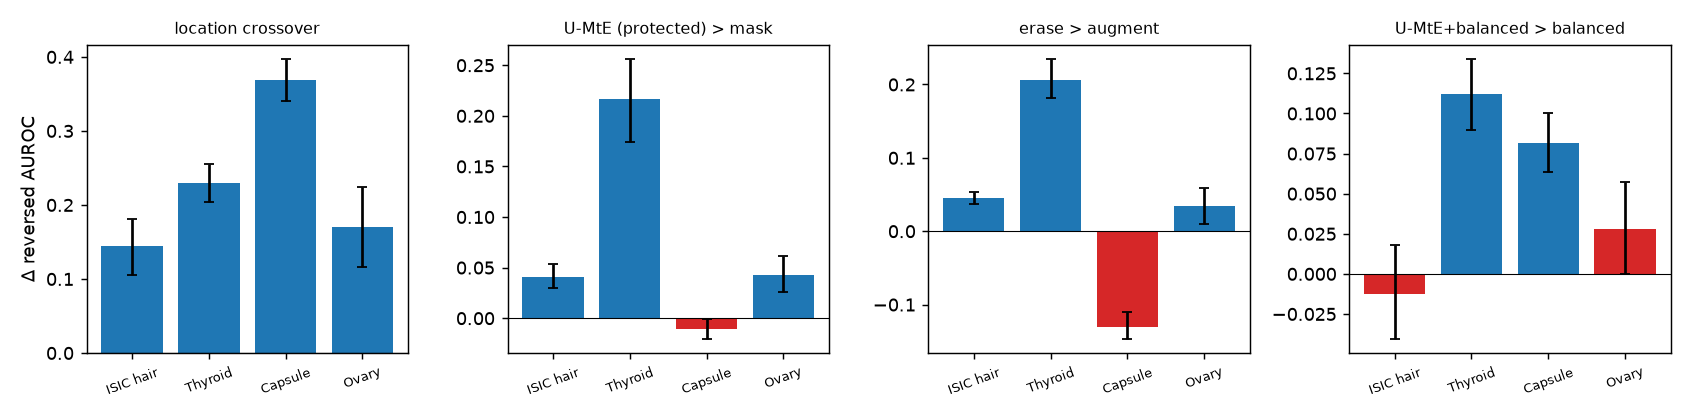
\includegraphics[width=\linewidth]{figures/primary_bars.png}
\caption{The 16 pre-registered headline tests (Holm-corrected; 12/16 supported).}\end{figure}
\begin{figure}[H]\centering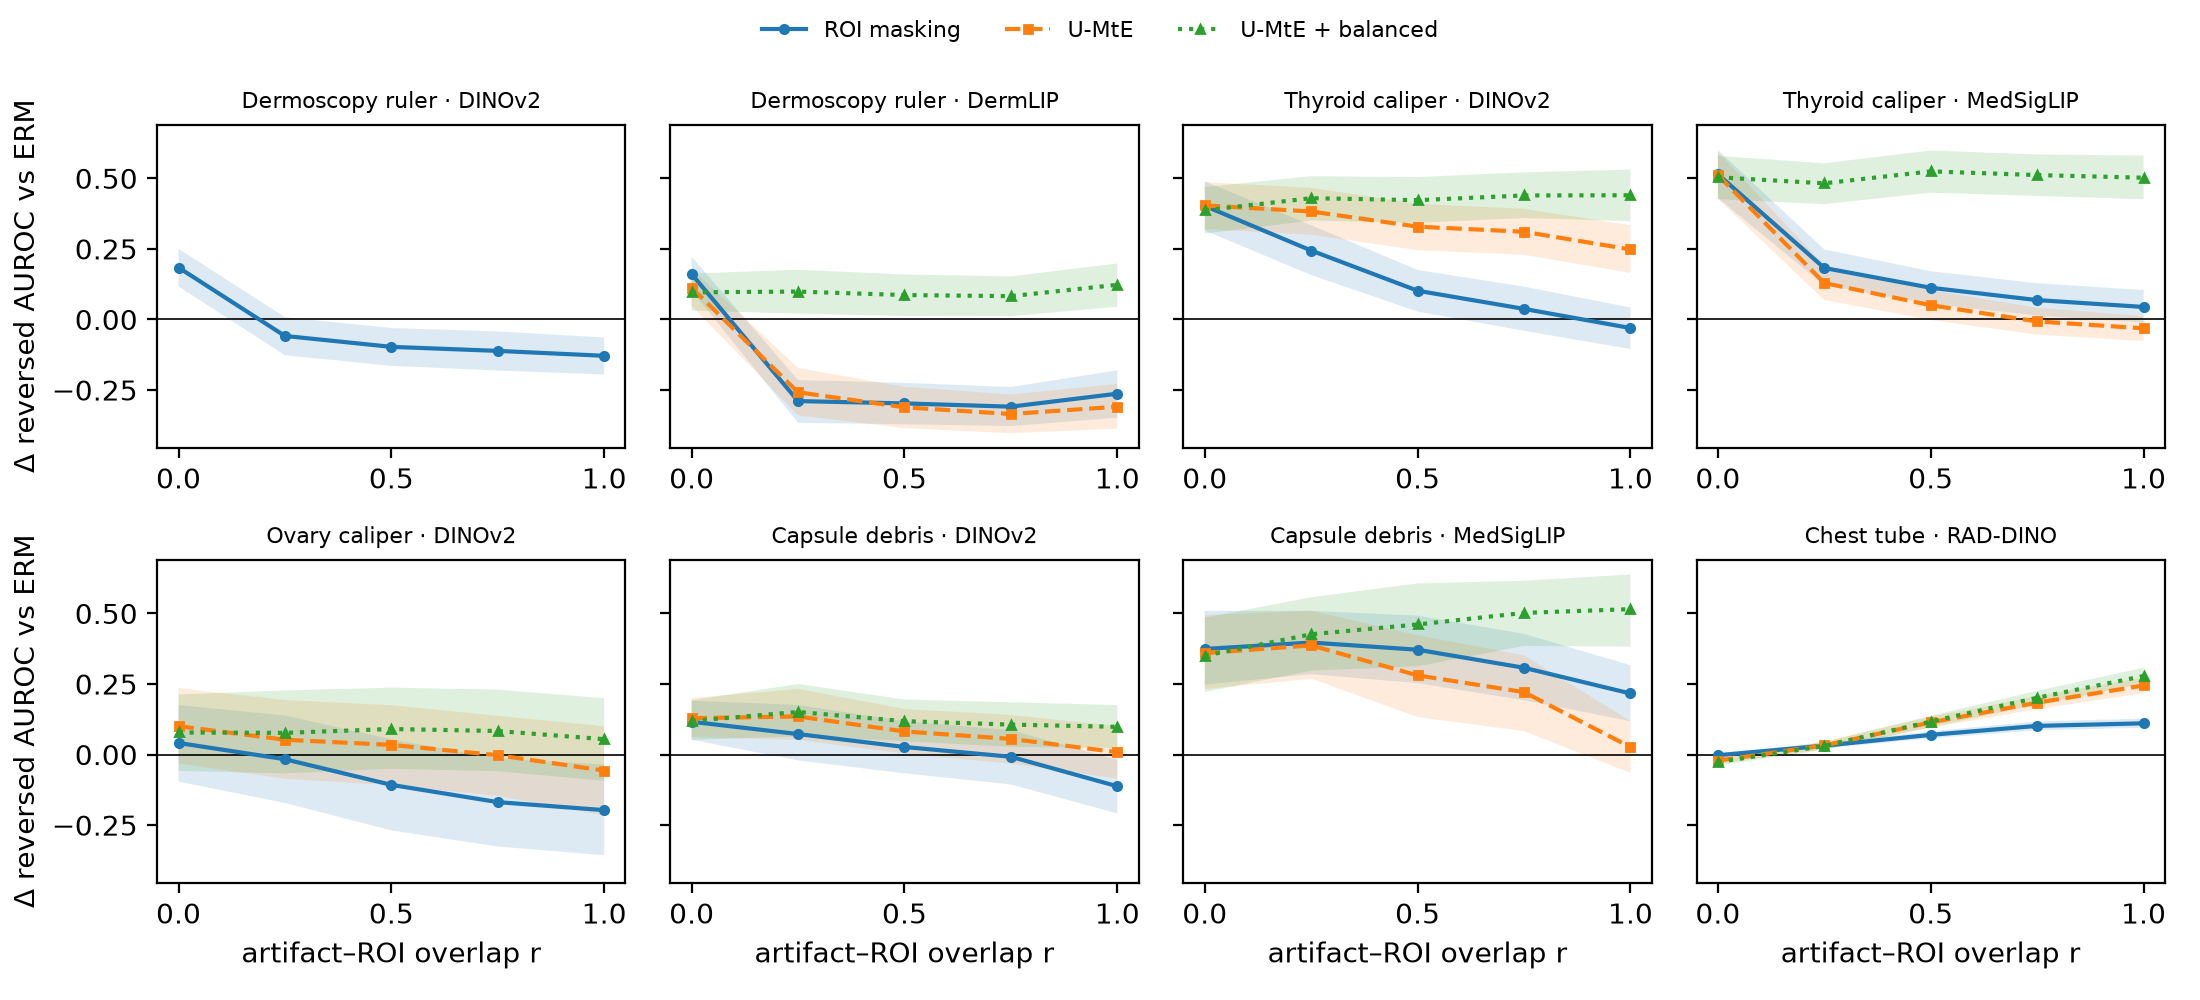
\includegraphics[width=\linewidth]{../paper/figures/dose_response.png}
\caption{Controlled sweeps: effect of each method versus ERM as the artifact moves into the ROI. Masking (blue) falls;
U-MtE + balancing (green) stays flat. The chest-tube panel is the boundary case in which the model ignores
out-of-lung tubes altogether.}\end{figure}

\subsection{On real, unaltered data}
% filled by the analysis once all natural-distribution runs finish
\mixed\ Thyroid (official split, 614 test images): masking lowers AUROC on shortcut-conflicting cases by $-0.10$
[$-0.14$, $-0.07$] and raises it on consistent cases ($+0.05$); U-MtE recovers half the loss, group balancing all of it.
Leave-one-hospital-out dermoscopy and capsule results: pending.


\subsection{Foundation models (no training)}
\plain{We asked the big medical AI models to classify using text prompts alone, with no training at all. Their answers
are already swayed by the artifacts, and masking helps them only when the artifact is outside the lesion---the same
location law, built into the models themselves.}
\ok\ Masking's effect on zero-shot hard-test accuracy is worse for in-ROI than out-of-ROI artifacts in all four tests
(thyroid $+0.10$, capsule $+0.05$, ovarian $+0.18$, hair $+0.05$ location gaps, all significant).

\no\ \textbf{Text-prompted erasure} (describe the artifact in words, erase that direction): a near no-op everywhere
($\le +0.008$). Our image-side method with the same model gains $+0.20$ (thyroid) and $+0.22$ (ovarian).

\subsection{Training the whole network}
\mixed\ Capsule (ResNet-50): masking harms in-ROI ($-0.28$), crossover $+0.58$. Thyroid (ViT-S): crossover $+0.17$
[$+0.07$, $+0.27$]. End-to-end U-MtE: $+0.14$ over masking with ResNet-50 on thyroid, no gain with ViT-S or on capsule.

\subsection{Why: a simple theory}
\begin{figure}[H]\centering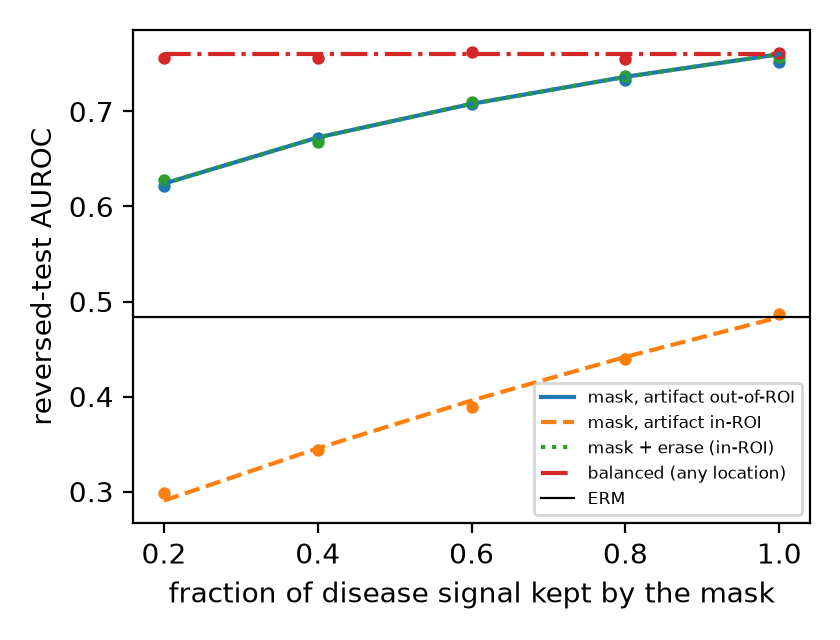
\includegraphics[width=.55\linewidth]{../paper/figures/theory.png}
\caption{$\mathrm{AUROC}_{\mathrm{rev}}=\Phi\big((S-\tilde A)/\sqrt{2(S+\tilde A)}\big)$ with disease signal $S$ and
effective artifact strength $\tilde A$ (lines) versus simulation (points).}\end{figure}
\plain{Masking an in-ROI artifact keeps the artifact and throws away other disease evidence, so the model leans on the
artifact even more. Erasing works unless the artifact looks like the disease. Re-balancing works wherever the artifact
sits.}
\begin{figure}[H]\centering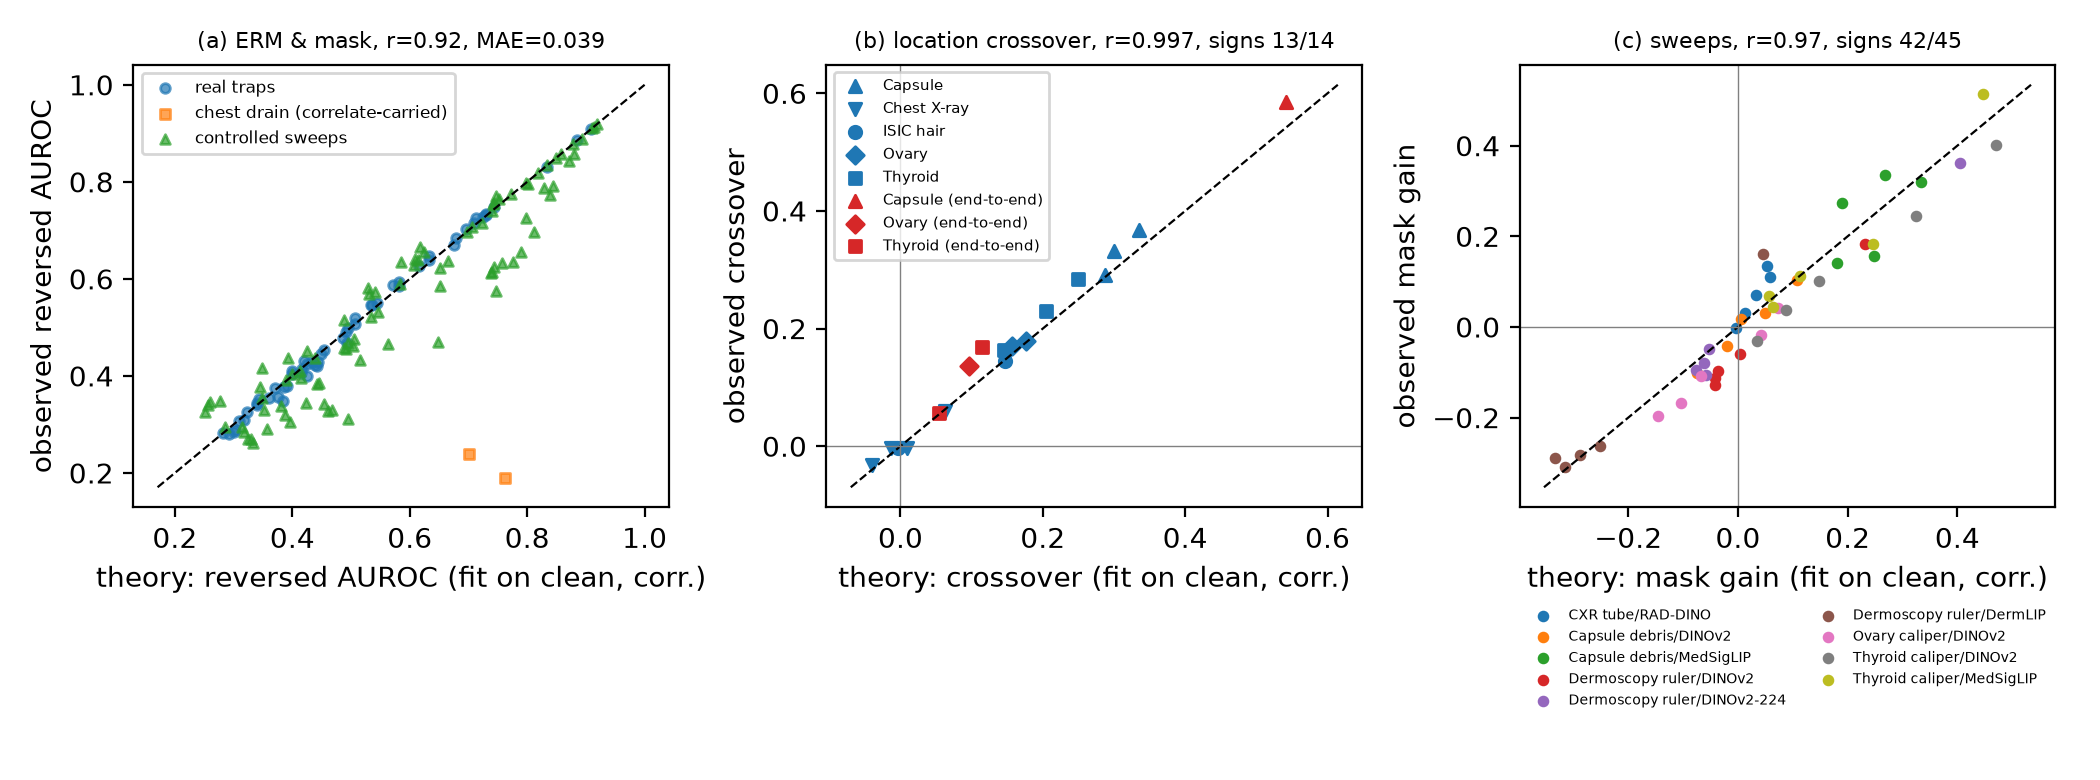
\includegraphics[width=\linewidth]{../paper/figures/theory_predict.png}
\caption{Pre-registered test on real models: the formula is fitted to each model's clean and correlated results, and
its hard-test (reversed) results are compared with the real ones, which it never saw.}\end{figure}
\plain{\ok\ The formula matches real models closely (left: average error 0.039; middle: the location gap, correlation
0.997). \no\ It misses the chest-drain models, where the shortcut lives in things that come with the drain (a treated
lung), which the formula cannot see. Because one of 14 location-gap signs (a value of $-0.002$) disagreed, our
pre-registered rule calls it a ``qualitative'' account.}

\begin{figure}[H]\centering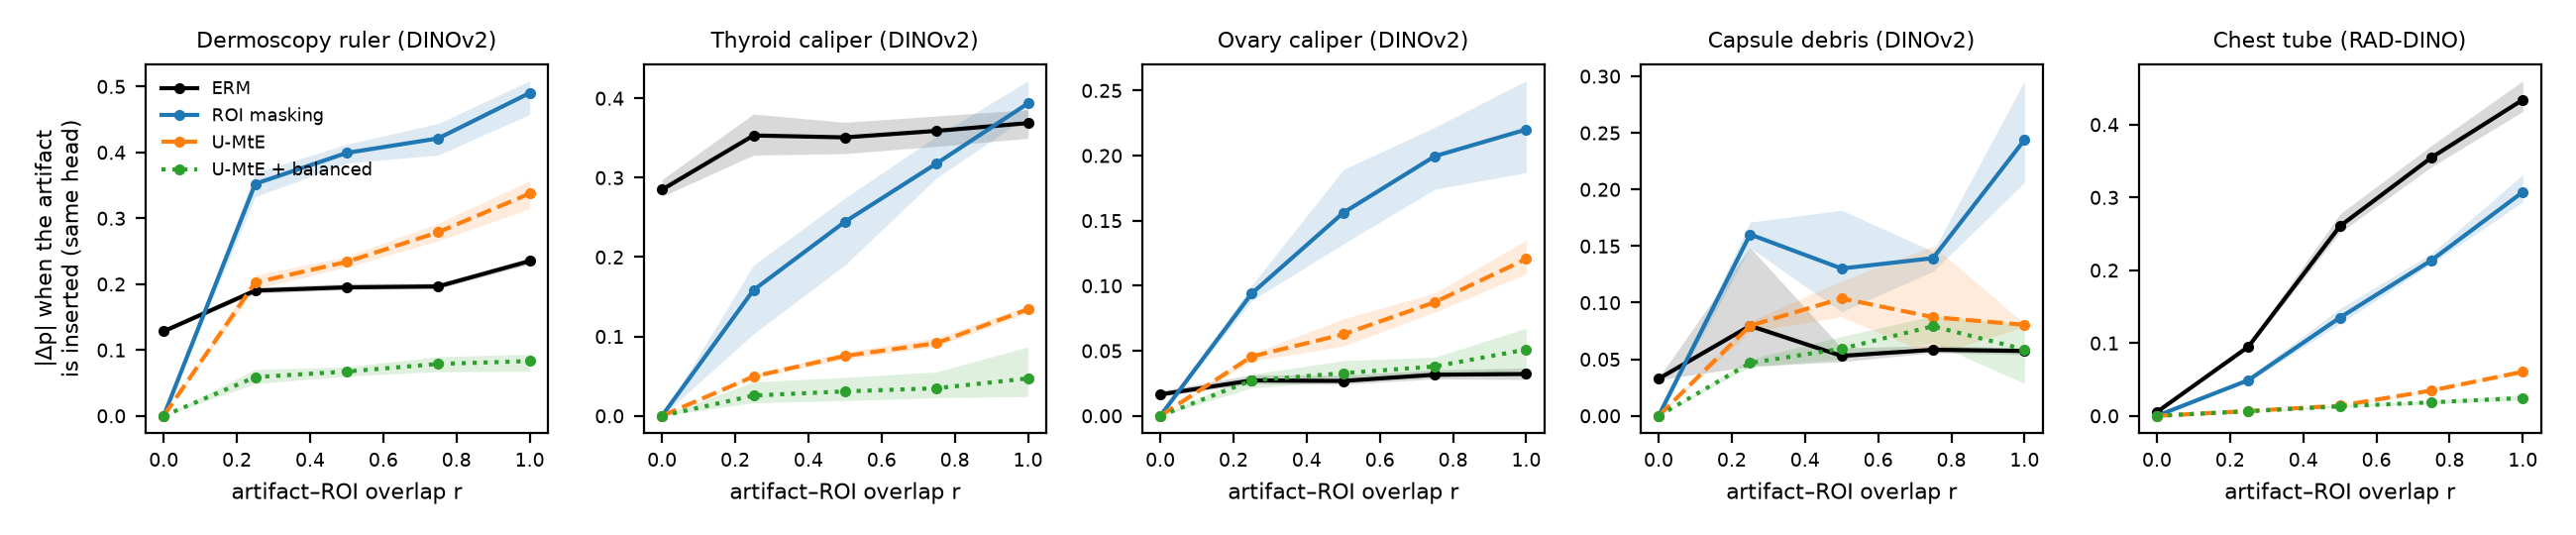
\includegraphics[width=\linewidth]{../paper/figures/mechanism.png}
\caption{Why masking fails in the ROI: how much the prediction changes when the artifact is added, versus how deep
inside the ROI it sits. Masking (blue) makes the model rely on an in-ROI artifact more; U-MtE (orange) and U-MtE with
balancing (green) remove that reliance.}\end{figure}

\subsection{Remedies compared}
\plain{Each column is a dataset/model; each row a method. Numbers are hard-test accuracy (in brackets: the fairer
summary that also penalises ``flipping''). Bold = best in the column.}
\begin{table*}[t]\centering\scriptsize
\caption{In-ROI artifacts (Trap~A): reversed-test AUROC, with min(reversed, correlated) in parentheses (penalises shortcut flipping). Best robust value per column in bold. Generated by \texttt{scripts/make\_main\_table.py}.}
\label{tab:main}
\begin{tabular}{llcccccccccc}
\toprule
Method & Needs & \rotatebox{90}{Hair/DINOv2} & \rotatebox{90}{Hair/DermLIP} & \rotatebox{90}{Thyroid/DINOv2} & \rotatebox{90}{Thyroid/MedSigLIP} & \rotatebox{90}{Thyroid/ConvNeXt} & \rotatebox{90}{Capsule/DINOv2} & \rotatebox{90}{Capsule/MedSigLIP} & \rotatebox{90}{Capsule/ConvNeXt} & \rotatebox{90}{Drain/RAD-DINO} & \rotatebox{90}{Drain/DINOv2} \\
\midrule
ERM & — & 0.49 (0.49) & 0.67 (0.67) & 0.29 (0.29) & 0.28 (0.28) & 0.35 (0.35) & 0.59 (0.59) & 0.59 (0.59) & 0.55 (0.55) & 0.19 (0.19) & 0.28 (0.28) \\
ROI masking & ROI & 0.45 (0.45) & 0.58 (0.58) & 0.40 (0.40) & 0.35 (0.35) & 0.36 (0.36) & 0.68 (0.68) & 0.70 (0.70) & 0.64 (0.64) & 0.24 (0.24) & 0.29 (0.29) \\
Mask + overlay augmentation & ROI & 0.46 (0.46) & – & 0.42 (0.42) & 0.38 (0.38) & 0.37 (0.37) & 0.70 (0.70) & 0.72 (0.72) & 0.65 (0.65) & 0.24 (0.24) & 0.29 (0.29) \\
\textbf{U-MtE (ours)} & ROI & 0.51 (0.51) & 0.51 (0.51) & 0.62 (0.62) & 0.55 (0.55) & 0.49 (0.49) & 0.57 (0.57) & 0.47 (0.47) & 0.56 (0.56) & 0.27 (0.27) & 0.28 (0.28) \\
\textbf{U-MtE, protected (ours)} & ROI + $Y$ of $A{=}0$ & 0.49 (0.49) & 0.59 (0.59) & 0.62 (0.62) & 0.61 (0.61) & 0.55 (0.55) & 0.67 (0.67) & 0.67 (0.67) & 0.64 (0.64) & 0.27 (0.27) & 0.28 (0.28) \\
Group-balanced & $A$ & 0.72 (0.72) & \textbf{0.81 (0.81)} & 0.68 (0.68) & 0.70 (0.70) & 0.66 (0.66) & 0.78 (0.78) & 0.81 (0.81) & 0.72 (0.72) & 0.54 (0.54) & 0.40 (0.40) \\
DFR & $A$ & \textbf{0.74 (0.74)} & 0.78 (0.78) & 0.74 (0.66) & 0.76 (0.72) & 0.71 (0.67) & 0.80 (0.80) & 0.80 (0.80) & 0.77 (0.77) & \textbf{0.68 (0.68)} & 0.55 (0.55) \\
Mask + DFR & ROI + $A$ & 0.69 (0.69) & – & 0.83 (0.74) & 0.81 (0.76) & 0.77 (0.72) & \textbf{0.88 (0.88)} & \textbf{0.90 (0.90)} & \textbf{0.86 (0.86)} & 0.65 (0.65) & \textbf{0.57 (0.57)} \\
\textbf{U-MtE + balanced (ours)} & ROI + $A$ & 0.70 (0.70) & 0.65 (0.65) & \textbf{0.79 (0.79)} & \textbf{0.79 (0.79)} & \textbf{0.74 (0.74)} & 0.86 (0.86) & 0.85 (0.85) & 0.80 (0.80) & 0.46 (0.46) & 0.44 (0.44) \\
\bottomrule
\end{tabular}
\end{table*}

\begin{itemize}[leftmargin=*]
\item \ok\ Erase beats augment with the same overlays: thyroid $+0.21$, hair $+0.05$, ovary $+0.04$; \no\ capsule $-0.13$.
\item \ok\ SPLINCE (closest published erasure, NeurIPS 2025) removes much disease signal and flips the shortcut on
capsule; U-MtE + balancing is more robust in 3 of 4 cohorts (not on chest drains, where DFR is best).
\item \mixed\ LaMa inpainting with artifact masks is strong; protected U-MtE matches it on thyroid without masks.
\item \mixed\ JTT (label-free): U-MtE wins on thyroid ($+0.20$) and ovary ($+0.14$); JTT wins on hair.
\item \mixed\ Selector: beats masking in all 5 cohorts, within 0.02 of the best candidate, beats DFR in 3/5.
\end{itemize}

\subsection{Robustness}
\ok\ Visual audit (40 images per cell) and re-runs with large-marker and strict-location definitions: the location
effect and the protected-U-MtE gain hold in every variant (\texttt{docs/SENSITIVITY\_ARTIFACT\_LABELS.md}).

\ok\ \textbf{Stricter patient-leakage control.} Thyroid, ovary and capsule datasets have no patient IDs. We also
grouped images whose foundation-model embeddings are near-identical (same patient or session) and re-ran everything:
11 of 12 main results are unchanged; \no\ only the small ovary ``erase beats augment'' advantage loses significance.

\ok\ \textbf{Model size.} Small, base and large DINOv2 models (21 M to 304 M parameters): the location effect holds
in all 9 dataset/size pairs, and U-MtE beats masking on thyroid and ovary at every size. Larger models cheat
\emph{more} on in-lesion calipers, so bigger models do not fix the problem.

\ok\ \textbf{Erasure rank.} U-MtE's thyroid gain is +0.18 to +0.22 whenever it erases 16 or more directions; the
protected version never hurts capsule by more than 0.01.

\no\ \textbf{Fine-tune, then erase.} Applying U-MtE after fully fine-tuning a ResNet-50 does not help (+0.004):
U-MtE is a tool for frozen foundation-model features.

\ok\ \textbf{Erase while fine-tuning.} Doing the erasure \emph{during} fine-tuning (on the network's own features, plus
making features and predictions ignore overlays) works for both a CNN and a transformer on thyroid: ResNet-50 +0.157,
ViT-S +0.143 over masking, with no artifact annotation. Ovary and capsule runs are pending (the GPU failed).

\mixed\ \textbf{Clinical metrics.} On the untouched thyroid test set, masking halves sensitivity at a fixed operating
point (0.73 $\to$ 0.35) while raising specificity (0.62 $\to$ 0.89); U-MtE recovers part of it and has the best AUPRC and
Brier score. On other hospitals and capsule, masking improves every metric.

\section{What did not work (and why it is still useful)}
\begin{itemize}[leftmargin=*]
\item \no\ ``Masking always harms in-ROI'' is not universal: in real thyroid/ovary/capsule it helps a little (removing
clutter); in chest X-rays the model ignores out-of-lung tubes. The universal claim is the location \emph{gap}.
\item \no\ U-MtE alone on capsule debris (resembles erosion fibrin) and with MedSigLIP in controlled sweeps.
\item \no\ SLAS (patch suppression): localises hair from 5 annotations but gives small classification gains.
\item \no\ Pseudo-group balancing without labels: helps thyroid only.
\item \no\ Datasets dropped: CANDID-PTX (no access), breast ultrasound (unreliable caliper labels), colonoscopy
(no reflection-free images), ink (too few), cardiomegaly lines (too few), pathology pen marks (unreliable masks).
\end{itemize}

\section{Reproduce and reuse}
\texttt{make data data\_extra}, then one target per experiment (\texttt{README.md}); every number is written by a script.
Tools: \texttt{python -m wtss.umte fit/embed} and \texttt{python -m wtss.slas fit/embed} for any backbone.

\section*{Data attribution}
ISIC Archive (CC BY-NC); HAM10000 (Tschandl et al.); Wegley et al.\ 2026 artifact masks; TN3K (Gong et al.) with TNCD
labels; MMOTU (Zhao et al., CC BY 4.0); SEE-AI (CC BY 4.0) and figshare 27645021; NIH ChestX-ray14; NEATX; RANZCR-CLiP.
Images appear as thumbnails for scientific illustration.
\end{document}
